\newpage
\subsection{Software}
Throughout the project, software was developed to aid in the electronic logging of water quality parameters. In this section, an overview of these software projects will be given. Script have been made in the Go programming language. This is due to the project producer having a lot of experience in Go and it being an excellent readable language for dealing with explicitly typed data.

\subsubsection{MCU Firmware}
As previously mentioned in \ref{mcu}, the Arduino environment was chosen to program the ATMega328P. The Arduino environment uses a C/C++ library which makes common input/output operations easier than writing the firmware "Bare-metal".\\

The firmware \cite{rwsuufirmware} is responsible for retrieving sensor values and logging them on a \gls{SD} card. Several libraries are used to aid in this process:

\begin{description}
   \item[DallasTemperature \cite{Dallas}] A library to read the temperature sensor
   \item[OneWire] \cite{OneWire} A library to access 1-Wire devices like the temperature sensor
   \item[DFRobot EC10] \cite{ec10} A library to read and calibrate the conductivity sensor
   \item[DFRobot PH] \cite{phlibrary} A library to read and calibrate the acidity sensor
   \item[DS1307RTC] \cite{DS1307RTC} A library to control the \gls{RTC} with the Time library
   \item[Time] \cite{timelibrary} A library for timekeeping functionality
   \item[SD] \cite{sdlibrary} A library for reading and writing to a SD card
\end{description}

Originally, the idea was to use CLion as the \gls{IDE}. As CLion is not well suited for Arduino development, PlatformIO \cite{platformio} is used in combination with VS Code instead as the \gls{IDE}. The code is still checked on MISRA standards using CLion. Documentation is generated from the source code via Doxygen. \cite{doxygen}
\newpage
\paragraph{SD Card} \label{sd}

The SD library is used to log the sensor values to the \gls{SD} card. An attempt was made to log the values in \gls{CSV} format to the \gls{SD} card, but string processing turned out to be quite resource intensive during testing. To save on resources, the decision was made to log the sensor values straight to a binary entry. Each binary entry has the following structure:

\begin{figure}[h]
\centering
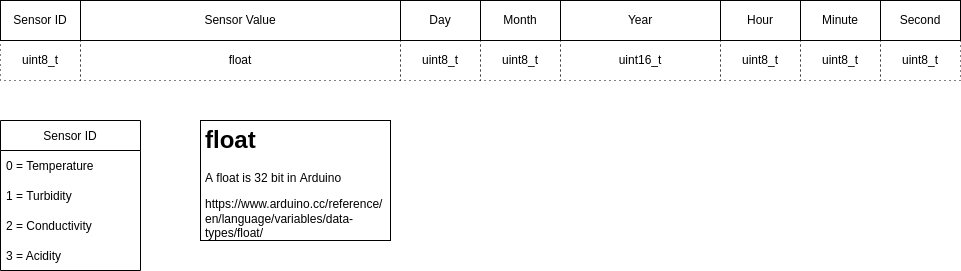
\includegraphics[scale=0.45]{070_design/software/61_datastructure.png}
\caption{Data structure of binary file}
\end{figure}

A new .DAT file with an unique filename is created on each boot. Entries are placed next to each other in the file. A Go \cite{golang} script has been made on the computer to convert the binary files to the desired \gls{CSV} format. \cite{dat2csv}

\paragraph{Sensors}

Every sensor has a simple and ordered interface interacting with the system:
\begin{enumerate}
  \item It has function that initializes the sensor that is called during the setup.
  \item It has a function that can calibrate the sensor. If necessary, it can be called at the end of the setup.
  \item It has a function that retrieves the value from the sensor that is called in the main loop
  \item It has an unique ID used when saving entries to the binary file.
\end{enumerate}

In the main loop, the sensor values are retrieved and stored on the \gls{SD} card.
\newpage
\subsubsection{Web Interface}
A web interface has been created using ThingsBoard \cite{thingsboard} to visualize the position of the drone and sensor data over time. This gives water quality researchers the tools to make sense of recorded data. Below, one can see the demo of the dashboard:

\begin{figure}[h]
\centering
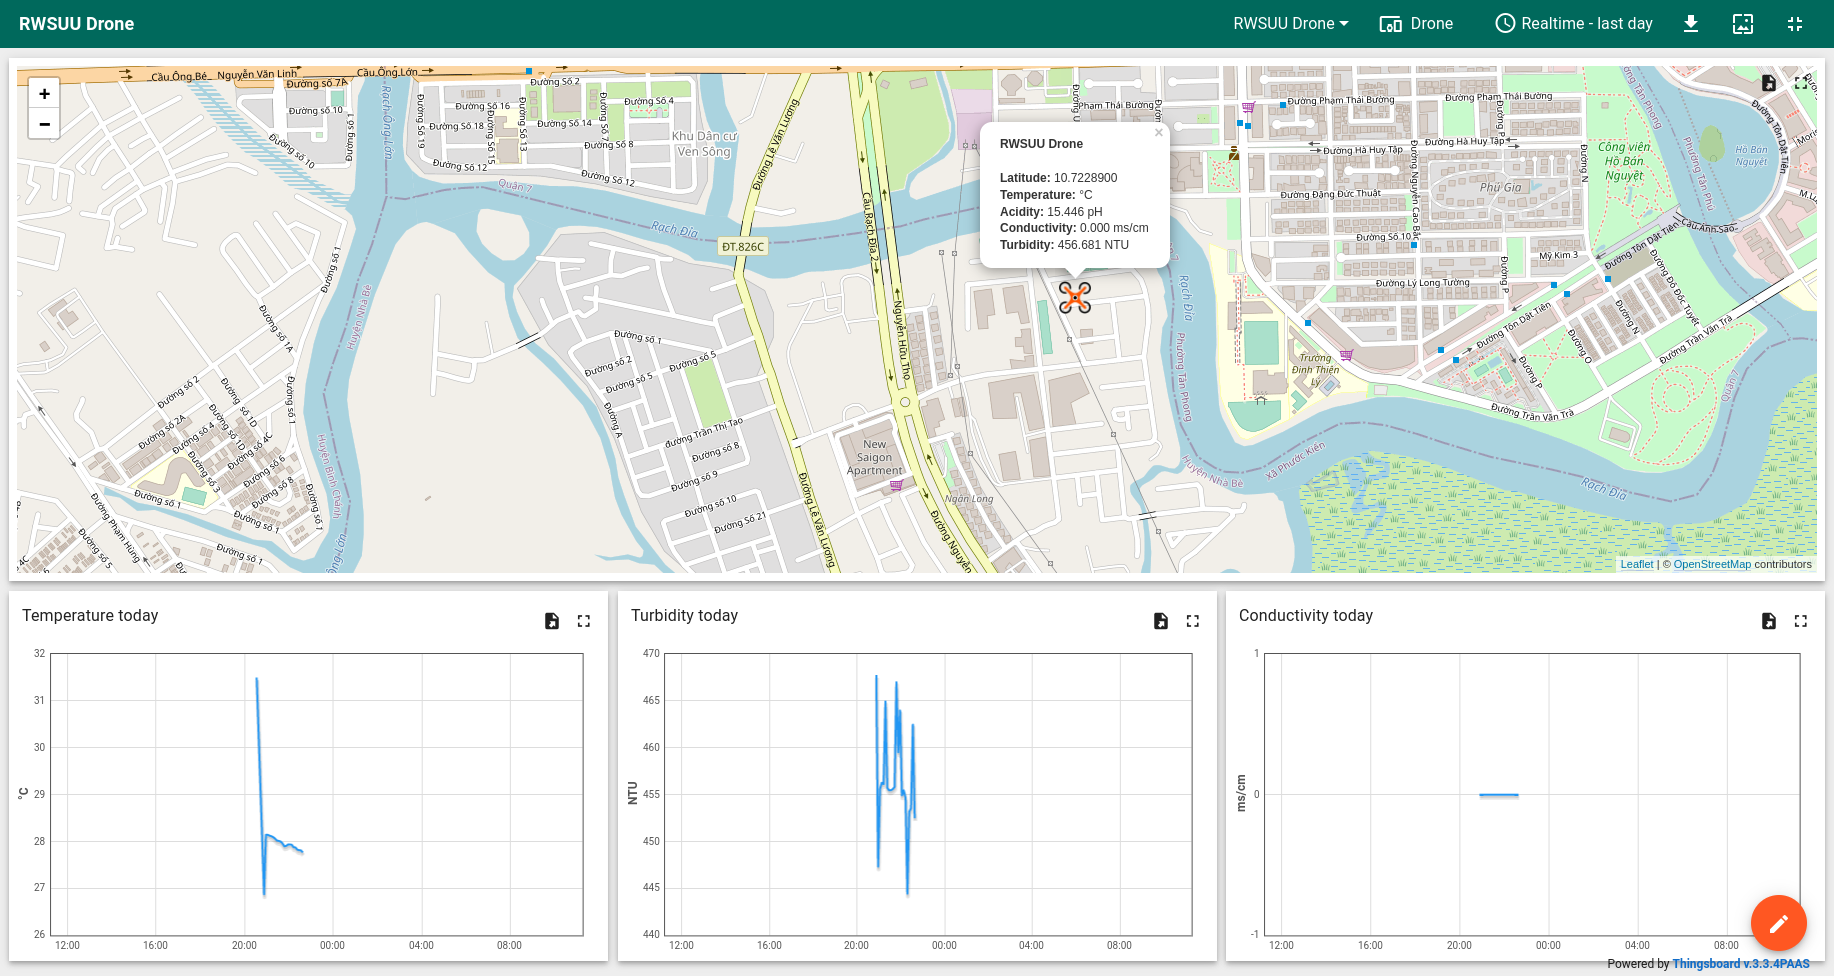
\includegraphics[scale=0.3]{070_design/software/63_dashboard.png}
\caption{Dashboard [own picture]}
\end{figure}

The communication of the sensor package and the drone is illustrated as follows:

\begin{figure}[h]
\centering
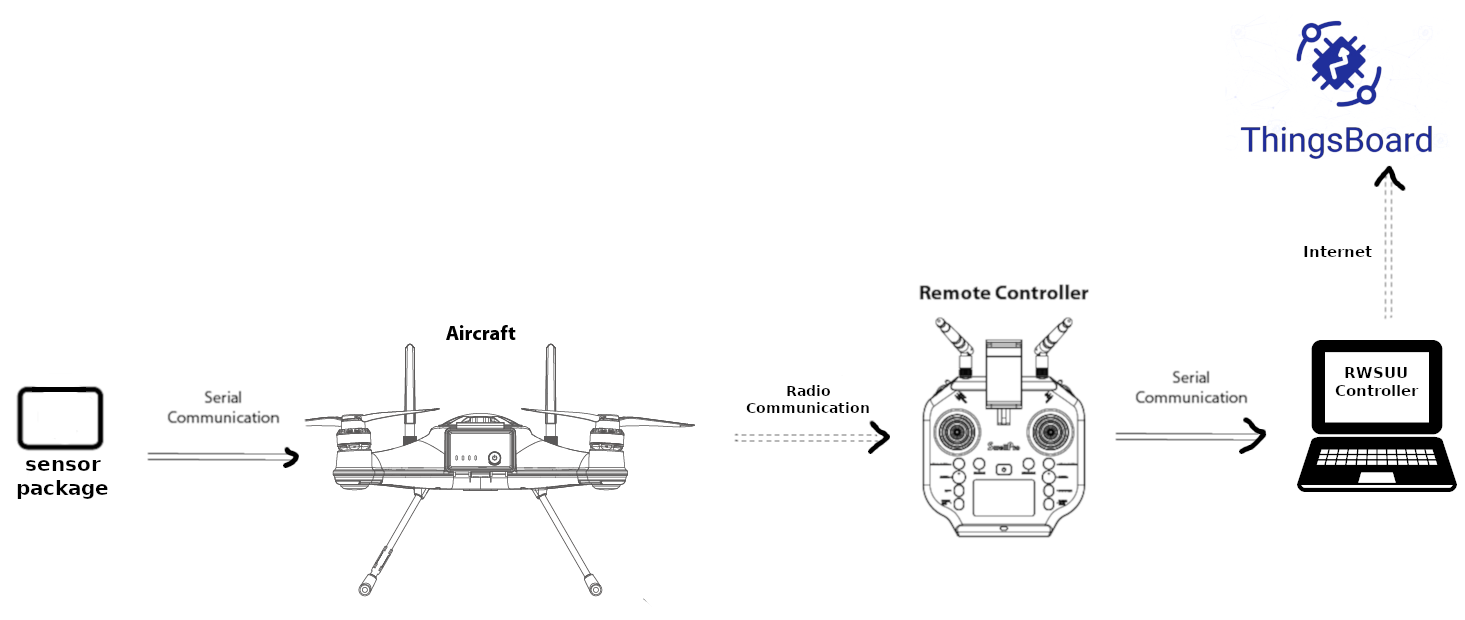
\includegraphics[scale=1]{070_design/software/62_comms.png}
\caption{Communication from sensor package to ThingsBoard [own edit from \cite{splashdronemanual}]}
\end{figure}

As one can see, the sensor package has a serial connection with the drone. The drone wirelessly passes through this serial connection to the remote controller. The data structure of the data passing through is the same as the data structure of each entry in the binary file on the SD Card, with a start bit added to indicate the beginning of the transmission. The remote controller has in turn a serial connection with the computer, and the computer is running a Golang script \cite{rwsuucontroller} to listen to this serial connection and pass this information to ThingsBoard.

